\subsection{Heterogeneous sensor systems}
\subsubsection{Heterogeneous capacitive arrays}
\begin{figure}[h]
\centering
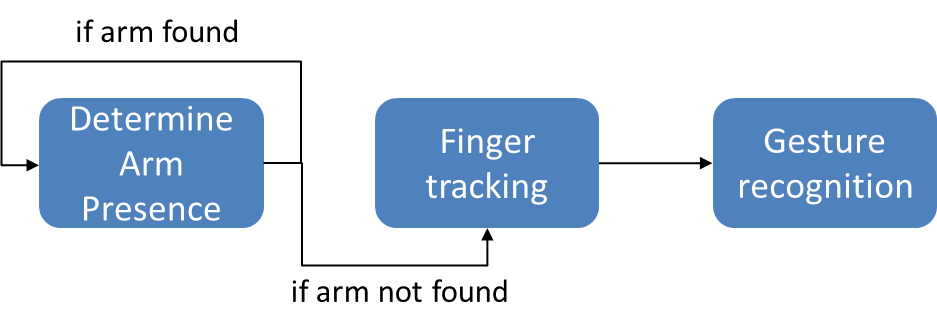
\includegraphics[width=0.4\textwidth]{images/armrest_dataproc}
\caption{Data processing pipeline of Active Armrest}
\label{fig:armrest_dataproc}
\end{figure}
%Figure 25 Data processing pipeline of Active Armrest
As we already mentioned, the Active Armrest electrodes are put into two groups. The data processing for both groups is distinctly different. In order to detect the presence of the arm using the two-electrode group a simple threshold on the accumulated values is used. The six sensor array in the front (touch area) is using the presented weighted average method to calculate finger positions. Additionally a threshold is used to distinguish one and two fingers. Overall there is a data processing pipeline as shown in Figure \ref{fig:armrest_proto}. The finger tracking and gesture recognition will be inactive until it is ensured that no arm is present. 

\subsubsection{Heterogeneous sensor fusion}
\begin{figure}[h]
\centering
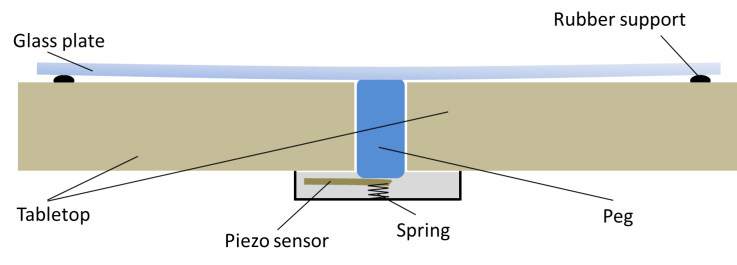
\includegraphics[width=0.7\textwidth]{images/captap_peg}
\caption{Suspended peg knock detection system for CapTap \cite{Braun2013ChairAid}}
\label{fig:captap_peg}
\end{figure}
%Figure 34 Suspended peg knock detection system for CapTap [80]
The hand location of the CapTap is similar to the methods presented for the MagicBox. We add the additional component of knock detection to provide selection events when touching the surface. Figure \ref{fig:captap_sketch} shows a sketch of the knock detection system. The table has a glass plate that is suspended on some rubber supports. In the center of the table we attach a small peg (enlarged in sketch) that creates a connection between the glass plate and a piezo sensor. If the glass plate starts vibrating from a touch we can measure this using the piezo sensor \cite{Braun2013ChairAid}. If a notable vibration is measured we are collecting the next 50 samples, resulting in a window of 250 milliseconds. To distinguish single and double knocks we calculate the weighted average within this window to get a measure for the distribution of sensor values within. If the average is closer to the beginning of the window the resulting event should be a single knock, and a double if the average is closer to the end of the window.
Hand localization and knock detection are working independently and are combined later in the software. It is reasonable to combine this, e.g. to ignore knock events that are occurring without a hand present. They may be indicative of a person doing a strong step close to the table.